\ifnum \Version=6
    \question[4] Consider the IVP $$\vec x \, ' = A\vec x, \quad A = \begin{pmatrix} 1&3\\3&1 \end{pmatrix}, \quad \vec x = \begin{pmatrix} x(t)\\y(t)\end{pmatrix}, \quad \vec x(0) = \begin{pmatrix} 2\\-2 \end{pmatrix}$$ The eigenvalues of $A$ are $\lambda_1 = 4$ and $\lambda_2 = -2$. 
    \begin{parts}
        \part Determine the eigenvectors of $A$. Please show your work. 
        
        \ifnum \Solutions=1 {\color{DarkBlue} 
        \textbf{Solutions:}
        For $\lambda_1$, with $\ast =$ not needed, we obtain
        \begin{align}
            A - \lambda_1 I = \begin{pmatrix} -3& 3\\\ast &\ast\end{pmatrix} \ \Rightarrow \ v_1 = \begin{pmatrix} 1\\1 \end{pmatrix}
        \end{align}
        For $\lambda_2$:
        \begin{align}
            A - \lambda_2 I = \begin{pmatrix} 3&3\\\ast& \ast \end{pmatrix} \ \Rightarrow \ v_2 = \begin{pmatrix} -1\\1 \end{pmatrix}
        \end{align}    
        } 
        \else 
            \vspace{6cm}   
        \fi        
        \part Use the given eigenvalues and the eigenvectors that you calculated in part (a) to solve the IVP.  
        
        \ifnum \Solutions=1 {\color{DarkBlue} 
        \textbf{Solutions:} the general solution to the DE is:
        $$\vec x = c_1 e^{-4t}\begin{pmatrix} -1\\1\end{pmatrix} + c_2e^{2t} \begin{pmatrix} 1\\1\end{pmatrix}$$
        Use initial condition:
        \begin{align}
            \begin{pmatrix} 2\\-2\end{pmatrix} &= c_1\begin{pmatrix}-1\\1 \end{pmatrix}+ c_2 \begin{pmatrix} 1\\1\end{pmatrix} \ \Rightarrow \ c_1 = -2, c_2 = 0 \ \Rightarrow \ 
            \vec x (t) = -2e^{2t} \begin{pmatrix} -1\\1\end{pmatrix}
        \end{align}
        } 
        \else 
        \vspace{7cm}
    \fi
    \part Sketch the phase portrait of the system on the axes below. Please indicate the direction of motion on your solution curves and draw the eigenspaces corresponding to real eigenvalues (if any). Please also label your axes. 
    
    \ifnum \Solutions=1 {\color{DarkBlue} 
    \textbf{Solutions:}
        \begin{center}
        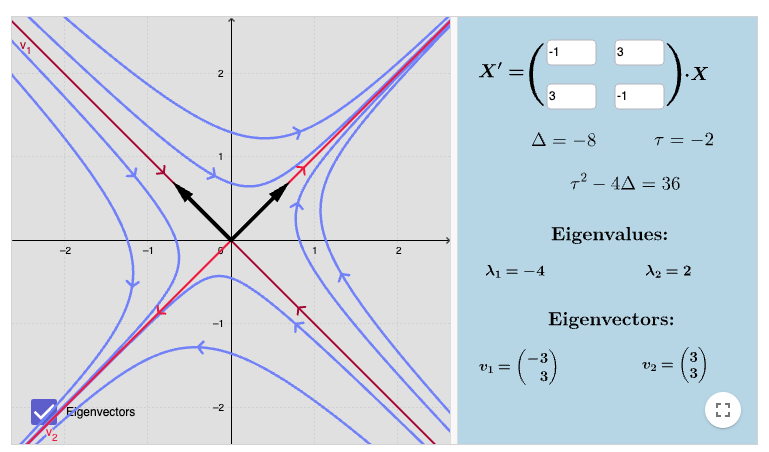
\includegraphics[width=5in]{Images/ImgPhasePlane1331.png}
        \end{center}         
    } 
    \else 
        \begin{center}
        \begin{tikzpicture}[scale=0.65]
        \draw[very thick, ->] (-3, 0) -- (3.25, 0);
        \draw[very thick, ->] (0, -3) -- (0, 3.25);
        \end{tikzpicture}
        \end{center}    
    \fi    

    \part Classify the critical point according to stability and type. 
    
    \ifnum \Solutions=1 {\color{DarkBlue} 
    \textbf{Solutions:} unstable saddle
    } 
    \else 
    \vspace{3cm}
    \fi
    
\end{parts}
\fi







\ifnum \Version=7
    \question[4] Consider the IVP $$\vec x \, ' = A\vec x, \quad A = \begin{pmatrix} -3&2\\2&-3 \end{pmatrix}, \quad \vec x = \begin{pmatrix} x(t)\\y(t)\end{pmatrix}, \quad \vec x(0) = \begin{pmatrix} 2\\-2 \end{pmatrix}$$ The eigenvalues of $A$ are $\lambda_1 = -1$ and $\lambda_2 = -5$. 
    \begin{parts}
        \part Determine the eigenvectors of $A$. Please show your work. 
        
        \ifnum \Solutions=1 {\color{DarkBlue} 
        \textbf{Solutions:}
        For $\lambda_1$, with $\ast =$ not needed, we obtain
        \begin{align}
            A - \lambda_1 I = \begin{pmatrix} -3& 3\\\ast &\ast\end{pmatrix} \ \Rightarrow \ v_1 = \begin{pmatrix} 1\\1 \end{pmatrix}
        \end{align}
        For $\lambda_2$:
        \begin{align}
            A - \lambda_2 I = \begin{pmatrix} 3&3\\\ast& \ast \end{pmatrix} \ \Rightarrow \ v_2 = \begin{pmatrix} -1\\1 \end{pmatrix}
        \end{align}    
        } 
        \else 
            \vspace{6cm}   
        \fi        
        \part Use the given eigenvalues and the eigenvectors that you calculated in part (a) to solve the IVP.  
        
        \ifnum \Solutions=1 {\color{DarkBlue} 
        \textbf{Solutions:} the general solution to the DE is:
        $$\vec x = c_1 e^{-t}\begin{pmatrix} 1\\1\end{pmatrix} + c_2e^{-5t} \begin{pmatrix} -1\\1\end{pmatrix}$$
        Use initial condition:
        \begin{align}
            \begin{pmatrix} 2\\-2\end{pmatrix} &= c_1\begin{pmatrix}1\\1 \end{pmatrix}+ c_2 \begin{pmatrix} -1\\1\end{pmatrix} \ \Rightarrow \ c_1 = 0, c_2 = -2 \ \Rightarrow \ 
            \vec x (t) = -2e^{-5t} \begin{pmatrix} -1\\1\end{pmatrix}
        \end{align}
        } 
        \else 
        \vspace{7cm}
    \fi
    \part Sketch the phase portrait of the system on the axes below. Please indicate the direction of motion on your solution curves and draw the eigenspaces corresponding to real eigenvalues (if any). Please also label your axes. 
    
    \ifnum \Solutions=1 {\color{DarkBlue}   
    \textbf{Solutions:}
        \begin{center}
        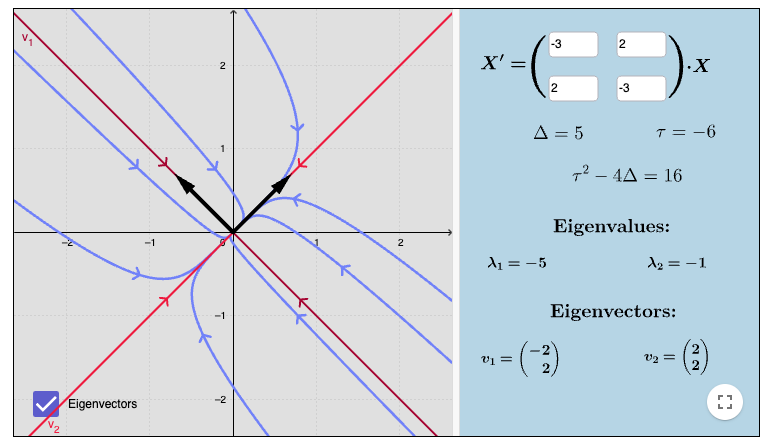
\includegraphics[width=5in]{Images/ImgPhasePlane3223.png}
        \end{center}         
    } 
    \else 
        \begin{center}
        \begin{tikzpicture}[scale=0.65]
        \draw[very thick, ->] (-3, 0) -- (3.25, 0);
        \draw[very thick, ->] (0, -3) -- (0, 3.25);
        \end{tikzpicture}
        \end{center}    
    \fi    

    \part Classify the critical point according to stability and type. 
    
    \ifnum \Solutions=1 {\color{DarkBlue} 
    \textbf{Solutions:} stable node
    } 
    \else 
    \vspace{3cm}
    \fi

\end{parts}
\fi